\documentclass[conference]{IEEEtran}

\usepackage[T1]{fontenc}
\usepackage{amsmath,amssymb,booktabs,graphicx,array}
\usepackage{xurl}
\usepackage[hidelinks]{hyperref}
\usepackage{listings}
\usepackage{xcolor}
\usepackage{tikz}
\usetikzlibrary{arrows.meta,positioning}
\graphicspath{{images/}}
\newcommand{\file}[1]{\path{#1}}
\lstset{basicstyle=\ttfamily\footnotesize,breaklines=true,columns=fullflexible,
 keepspaces=true,showstringspaces=false,frame=single}

\usepackage{placeins}

\newcommand{\ProjectAuthorNames}{Mohammadilyas Patel, Shaik Sifat Ahmed, Abhinay}
\newcommand{\ProjectInstitution}{Indian Institute of Information Technology,\\Design and Manufacturing, Kancheepuram}
\newcommand{\ProjectLocation}{Chennai 600127, India}
\newcommand{\ProjectTeam}{Team 19}
\newcommand{\ProjectRepo}{https://github.com/mdilyas-27/cns_project_team_19}

\hypersetup{pdfauthor={\ProjectAuthorNames},pdftitle={Exploring and Enhancing Placement of Intrusion Detection Systems in RPL: A Federated Learning-Based Approach}}

\title{Exploring and Enhancing Placement of Intrusion Detection Systems in RPL: A Federated Learning-Based Approach}

\author{
    \IEEEauthorblockN{Mohammadilyas Patel}
    \IEEEauthorblockA{
        cs23b1078@iiitdm.ac.in\\
        Dept. of CSE, Team 19\\
        IIITDM Kancheepuram\\
        Chennai 600127, India
    }
    \and
    \IEEEauthorblockN{Shaik Sifat Ahmed}
    \IEEEauthorblockA{
        cs23b1035@iiitdm.ac.in\\
        Dept. of CSE, Team 19\\
        IIITDM Kancheepuram\\
        Chennai 600127, India
    }
    \and
    \IEEEauthorblockN{Abhinay}
    \IEEEauthorblockA{
        cs23i1009@iiitdm.ac.in\\
        Dept. of CSE, Team 19\\
        IIITDM Kancheepuram\\
        Chennai 600127, India
    }
}

\begin{document}
\maketitle

\begin{abstract}
Where should an intrusion detection engine actually sit inside a multi-hop RPL wireless mesh? Most published papers benchmark machine learning classifiers assuming a central sink inspects all packets. In real low-power deployments, that assumption fails. Packets dropped or tampered with eight hops away never reach the border router. In this course project, we analyze 31,626 Cooja simulation traces across a 10-level grid of Zolertia Z1 motes to study this placement dilemma. Our experiments show that placing an IDS only at the root (CIDwL) leaves downstream nodes completely exposed. For Blackhole attacks, detection accuracy collapses from 98.8\% at hop 1 down to 51.5\% at hop 8. Enlisting 9 distributed monitors (CIDwG) restores detection to 99.4\%. However, forwarding 35 feature values every minute generates 378~kB of telemetry per round. This load severely congests the 250~kbps 802.15.4 channel. To resolve this trade-off, we implement Federated Intrusion Detection (FedID). Motes train local XGBoost models and share only tree split weights. During testing, FedID requires zero bytes of communication. Sharing a modest 10\% slice of local data corrects non-IID traffic skew across network tiers, achieving 95.7\% Blackhole detection on RPL data and 99.60\% accuracy on the CICIoT2023 benchmark. Finally, we propose and simulate DR-FedID for upcoming iterations. DR-FedID rotates monitors dynamically to catch relocating attackers, raising detection from 72.00\% to 86.15\%. It also applies Multi-Krum aggregation to neutralize poisoned updates, restoring accuracy from 56.19\% back to 67.96\%.
\end{abstract}

\begin{IEEEkeywords}
RPL, Low-Power and Lossy Networks, Intrusion Detection System, Placement Strategy, Federated Learning, XGBoost, Non-IID Traffic, Byzantine Resilience.
\end{IEEEkeywords}

\section{Introduction}
When deploying low-power wireless meshes for environmental monitoring or industrial telemetry, network engineers face severe hardware constraints. The sensor motes in these networks---such as the Zolertia Z1 or TelosB platforms---typically feature 16-bit MSP430 microcontrollers, only 8 to 10~kB of RAM, and low-rate CC2420 radio chips operating over IEEE 802.15.4 at a peak bitrate of 250~kbps. Batteries must last for years. Routing in these networks is governed by the Routing Protocol for Low-Power and Lossy Networks (RPL, RFC 6550)~\cite{alexander2012rpl}, which builds a destination-oriented directed acyclic graph (DODAG) rooted at a 6LoWPAN border router (6LBR). Links remain notoriously lossy.

While link-layer cryptographic mechanisms protect against unauthorized external nodes, they offer little defense against compromised insider motes. An adversary holding valid cryptographic keys can easily falsify routing advertisements or drop forwarded application packets without violating link-layer checks. To detect such misbehavior, researchers have proposed numerous machine learning and deep learning intrusion detection systems (IDS). However, existing research exhibits a recurring oversight: studies almost universally assume an idealized central observer with complete visibility across all network traffic. That assumption fails in practice.

In a physical multi-hop mesh, this central visibility does not exist. If a compromised node located seven hops from the sink silently drops packets, those dropped packets never reach the root. The border router observes only normal ambient traffic from its immediate neighbors. This creates a complete blind spot. The reasons are physical.

In this course project, we systematically evaluate three fundamental IDS placement architectures originally analyzed by Yilmaz, Sen, and Aydogan~\cite{yilmaz2025exploring}: root-only monitoring (CIDwL), multi-node feature streaming (CIDwG), and distributed alarm voting (DCID). We structure our investigation around three core research questions:
\begin{enumerate}
    \item \textit{RQ1:} How severely does centralized root monitoring degrade as the attacking node moves deeper into the DODAG hierarchy?
    \item \textit{RQ2:} What minimum monitor density is required to restore full visibility, and what transmission load does it impose on 802.15.4 radio links?
    \item \textit{RQ3:} Can local voting consensus suppress false alarms without overwhelming channel capacity?
\end{enumerate}
These questions guide our evaluation.

Beyond evaluating these classical paradigms, we implement and test Federated Intrusion Detection (FedID), which replaces raw feature streaming with local XGBoost parameter exchanges, eliminating runtime packet overhead entirely. Testing communication is zero. We then propose and simulate a novel extension---Dynamic and Resilient FedID (DR-FedID)---incorporating routing-churn monitor rotation, Multi-Krum Byzantine aggregation, and Local Differential Privacy for upcoming project iterations.

\section{Related Work}
Over the past decade, many researchers have explored machine learning techniques to identify routing disruptions in RPL networks. For example, Verma and Ranga developed ELNIDS using ensemble classifiers~\cite{verma2019elnids}, while Napiah et al. designed decision trees to inspect compressed 6LoWPAN headers~\cite{napiah2018compression}. Shukla applied K-means clustering to localize wormhole attacks~\cite{shukla2017mlids}, and Airehrour et al. proposed trust-based forwarding mechanisms. Despite their varying classifiers, these systems share a common assumption: they rely on centralized feature collection at the border router.

As Raza et al. demonstrated in their work on SVELTE~\cite{raza2013securing}, forwarding raw routing statistics across multiple hops quickly drains node batteries and leads to severe packet loss. While distributed trust schemes (such as those by Medjek et al.~\cite{medjek2017trust} and Khan et al.~\cite{khan2017trust}) offload evaluation to neighboring motes, maintaining neighbor trust tables consumes substantial memory on MSP430 motes.

To overcome the communication bottleneck of centralized learning, federated learning (FL) has emerged as an attractive alternative. McMahan et al. introduced Federated Averaging (FedAvg) to train models across distributed devices without sharing private data~\cite{mcmahan2017communication}. Abbas et al. reviewed FL applications across IoT settings~\cite{abbas2023fl}. However, multi-hop RPL topologies introduce unique spatial challenges. Nodes adjacent to the 6LBR forward aggregated traffic from dozens of downstream children, whereas leaf nodes process only localized telemetry. This generates non-identical (non-IID) data distributions across network tiers. Yilmaz, Sen, and Aydogan~\cite{yilmaz2025exploring} addressed this problem by coupling federated averaging with tree-based XGBoost models and a local sample-sharing heuristic. Their study forms the empirical baseline for our work.

\section{Problem Formulation and Methodology}
\subsection{Routing Protocol and Threat Formulation}
RPL establishes network topology through ICMPv6 control messages. DODAG Information Object (DIO) packets advertise downward routes and topological Rank. DODAG Information Solicitation (DIS) packets request configuration details from neighbors. Destination Advertisement Object (DAO) packets register upward paths toward the root. In normal operation, a node computes its Rank via the Minimum Rank with Hysteresis Objective Function (MRHOF) based on Expected Transmission Count (ETX), ensuring Rank increases monotonically with distance from the sink.

We analyze seven prominent routing attacks executed across network tiers: Decreased Rank (DR), where an adversary advertises a false low Rank to capture parent status; Increased Version (IV), which forces global graph rebuilds; Blackhole (BH), dropping 100\% of forwarded traffic; Selective Forwarding (SF), dropping packets probabilistically; DIS Flooding (DI) and DIO Flooding (HF), which exhaust neighbor batteries through Trickle resets; and Wormhole (WP), which tunnels packets via out-of-band links.

\subsection{Architectural Placement Models}
We evaluate three distinct structural paradigms for placing the IDS engine. In Centralized with Local Information (CIDwL), detection runs exclusively on the root border router (ID: 0) using promiscuous packet capture:
\begin{equation}
    y_{\text{pred}}(t) = M_{\text{root}}(X_{\text{root}}(t))
\end{equation}
In Centralized with Global Information (CIDwG), $K$ distributed collaborator nodes across the DODAG extract 35 routing features every 60 seconds and forward them to the root:
\begin{equation}
    y_{\text{pred}}(t) = M_{\text{root}}([X_{\text{root}}(t), X_1(t), \dots, X_K(t)])
\end{equation}
In Distributed Collaborative IDS (DCID), every collaborator runs an independent local classifier, computes a binary alarm, and sends a 1-bit vote to the root:
\begin{equation}
    y_{\text{global}} = \mathbb{I}\left( \frac{1}{K} \sum_{k=1}^K a_k \ge \theta \right)
\end{equation}
The border router triggers an alarm if the fraction of positive votes meets threshold $\theta$.

\subsection{Federated Intrusion Detection (FedID)}
FedID replaces raw feature transmission with local model training and parameter aggregation. Collaborator motes train local XGBoost decision trees on their own 60-second traffic windows. The root server computes the weighted average of tree parameters:
\begin{equation}
    W_{\text{global}}(t+1) = \sum_{k=1}^K \frac{n_k}{N} W_k(t+1)
\end{equation}
During inference, each node executes the trained global model autonomously. Testing communication overhead is strictly zero.

\begin{figure}[htbp]
  \centering
  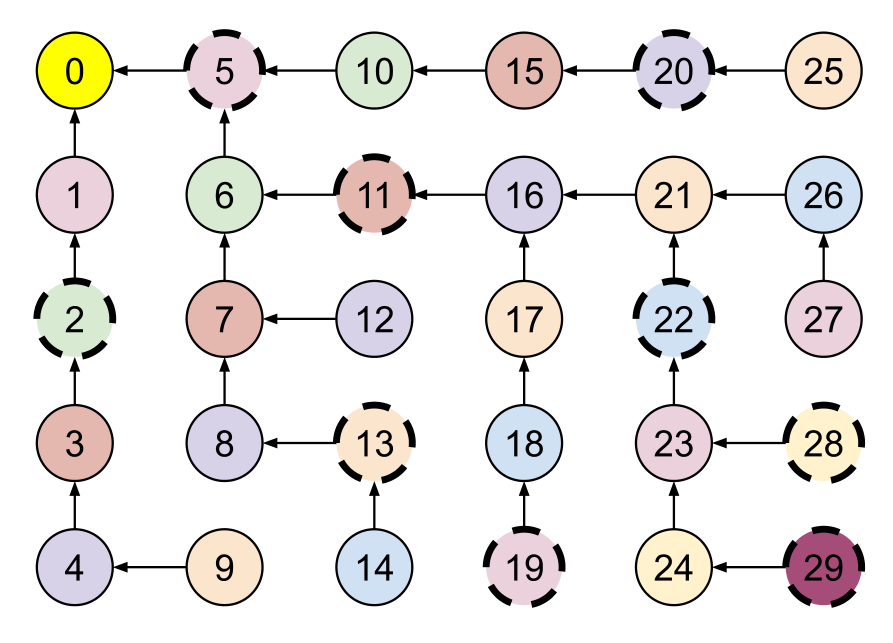
\includegraphics[width=0.88\columnwidth]{fig1_network_topology.png}
  \caption{Evaluated 30-node multi-hop grid DODAG topology partitioned across 10 hierarchical levels (Hop 0 to 9) [3].}
  \label{fig:topology}
\end{figure}

\begin{figure}[htbp]
  \centering
  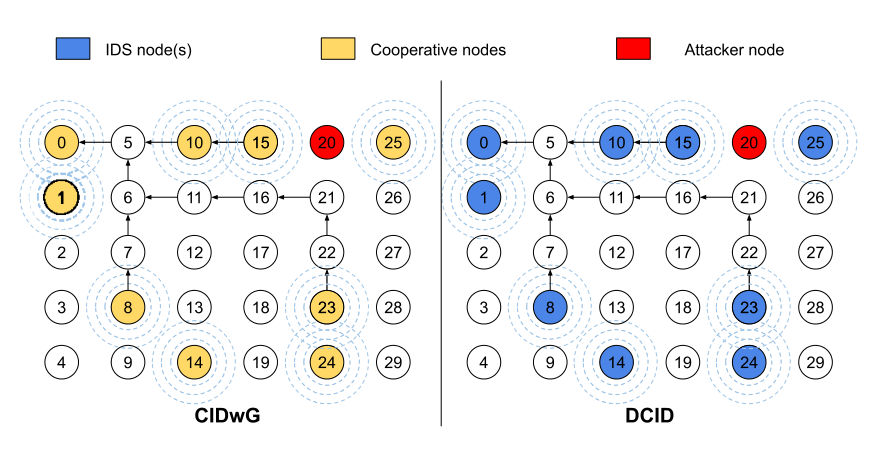
\includegraphics[width=0.88\columnwidth]{fig2_scenario_collaborators.png}
  \caption{Collaborator deployment across DODAG levels for CIDwG and DCID configurations [3].}
  \label{fig:collaborators}
\end{figure}

\section{Data and Experimental Protocol}
\subsection{Simulation Environment and Hardware Specifications}
All simulation runs were executed in Cooja within Contiki OS 2.7. The setup simulates 30 Zolertia Z1 sensor motes deployed across an 80~m $\times$ 100~m grid arranged in a 10-level hierarchy (Hops 0 to 9, shown in Fig.~\ref{fig:topology}). The motes emulate 16-bit MSP430 microcontrollers with 8~kB of RAM and 92~kB of ROM. Wireless channels use the Unit Disk Graph Model (UDGM) with distance-based path loss and a 25~m transmission radius. Motes send periodic UDP packets toward the sink every 15 seconds. The experimental dataset comprises 31,626 distinct 5-hour simulation runs. Table~\ref{tab:sim_params} summarizes the configuration parameters.

\begin{table}[htbp]
  \centering
  \caption{SIMULATION CONFIGURATION PARAMETERS [3]}
  \label{tab:sim_params}
  \begin{tabular}{ll}
    \toprule
    \textbf{Parameter} & \textbf{Experimental Value} \\
    \midrule
    Network OS & Contiki OS 2.7 (Cooja Simulator) \\
    Target Mote & Zolertia Z1 (MSP430, 8KB RAM) \\
    Radio Model & UDGM: Distance Loss (25m TX range) \\
    Topology Area & 100 m $\times$ 80 m Grid (30 nodes, 10 levels) \\
    RPL Objective & MRHOF with ETX Link Metric \\
    Traffic Pattern & Periodic UDP (1 packet per 15 s) \\
    Simulation Run & 5 hours per scenario (31,626 runs) \\
    Feature Window & 60-second sliding time windows \\
    Baseline ML & Random Forest (Scikit-Learn, 10-fold CV) \\
    FL Framework & Flower atop XGBoost ($\eta=0.3$, depth=6) \\
    \bottomrule
  \end{tabular}
\end{table}

\subsection{Feature Extraction and Non-IID Distribution}
Features are computed over 60-second non-overlapping sliding windows. The resulting 35-dimensional feature vector captures control packet counts (DIO, DIS, DAO sent/received), packet transmission and drop ratios, Rank stability, and inter-arrival timing statistics. Because traffic volume scales with proximity to the sink, feature distributions vary dramatically across DODAG tiers, producing pronounced non-IID conditions.

\subsection{Benchmark Validation on CICIoT2023}
To verify that our models generalize beyond simulated RPL environments, we additionally evaluate performance on the real-world CICIoT2023 dataset~\cite{neto2023ciciot2023}. Collected across 105 physical IoT devices, this dataset covers 33 attack types grouped into 7 categories (DDoS, DoS, Recon, Web, Brute Force, Spoofing, Mirai).

\section{Experimental Results and Discussion}
\subsection{RQ1: Spatial Detection Degradation in CIDwL}
When the IDS resides solely at the root node, detection capability degrades sharply as the attacker moves further away. Table~\ref{tab:cidwl} and Fig.~\ref{fig:heatmap} illustrate this effect. For a Blackhole attacker at Level 1, root detection achieves 98.8\% accuracy. When the attacker relocates to Level 8, Blackhole detection plummets to 51.5\%---a 47.3\% decline. The explanation is physical: because dropped packets never cross radio hops to the root, the border router has no data to inspect.

Selective Forwarding detection remains poor across all depths (58.0\% at Level 1, 51.2\% at Level 9). DIS Flooding accuracy falls from 96.7\% to 50.3\% due to localized Trickle resets. In contrast, Increased Version attacks maintain 99.3\% accuracy at all depths because version churn propagates network-wide. In answer to RQ1, centralized root monitoring is structurally incapable of securing multi-hop meshes against downstream attacks.

\begin{table}[htbp]
  \centering
  \caption{CIDWL DETECTION ACCURACY AT ROOT NODE (ID:0) [3]}
  \label{tab:cidwl}
  \begin{tabular}{ccccccc}
    \toprule
    \textbf{Atk} & \textbf{L1} & \textbf{L3} & \textbf{L5} & \textbf{L7} & \textbf{L9} & \textbf{Max Drop} \\
    \midrule
    BH & 0.988 & 0.533 & 0.530 & 0.540 & 0.562 & 0.473 \\
    SF & 0.580 & 0.528 & 0.540 & 0.508 & 0.512 & 0.075 \\
    DI & 0.967 & 0.557 & 0.520 & 0.570 & 0.503 & 0.495 \\
    DR & 0.500 & 0.568 & 0.535 & 0.528 & 0.538 & 0.132 \\
    HF & 1.000 & 0.802 & 0.582 & 0.592 & 0.553 & 0.483 \\
    IV & 0.998 & 1.000 & 0.998 & 0.997 & 0.993 & 0.007 \\
    WP & 0.927 & 0.517 & 0.510 & 0.522 & 0.493 & 0.433 \\
    \bottomrule
  \end{tabular}
\end{table}

\begin{figure}[htbp]
  \centering
  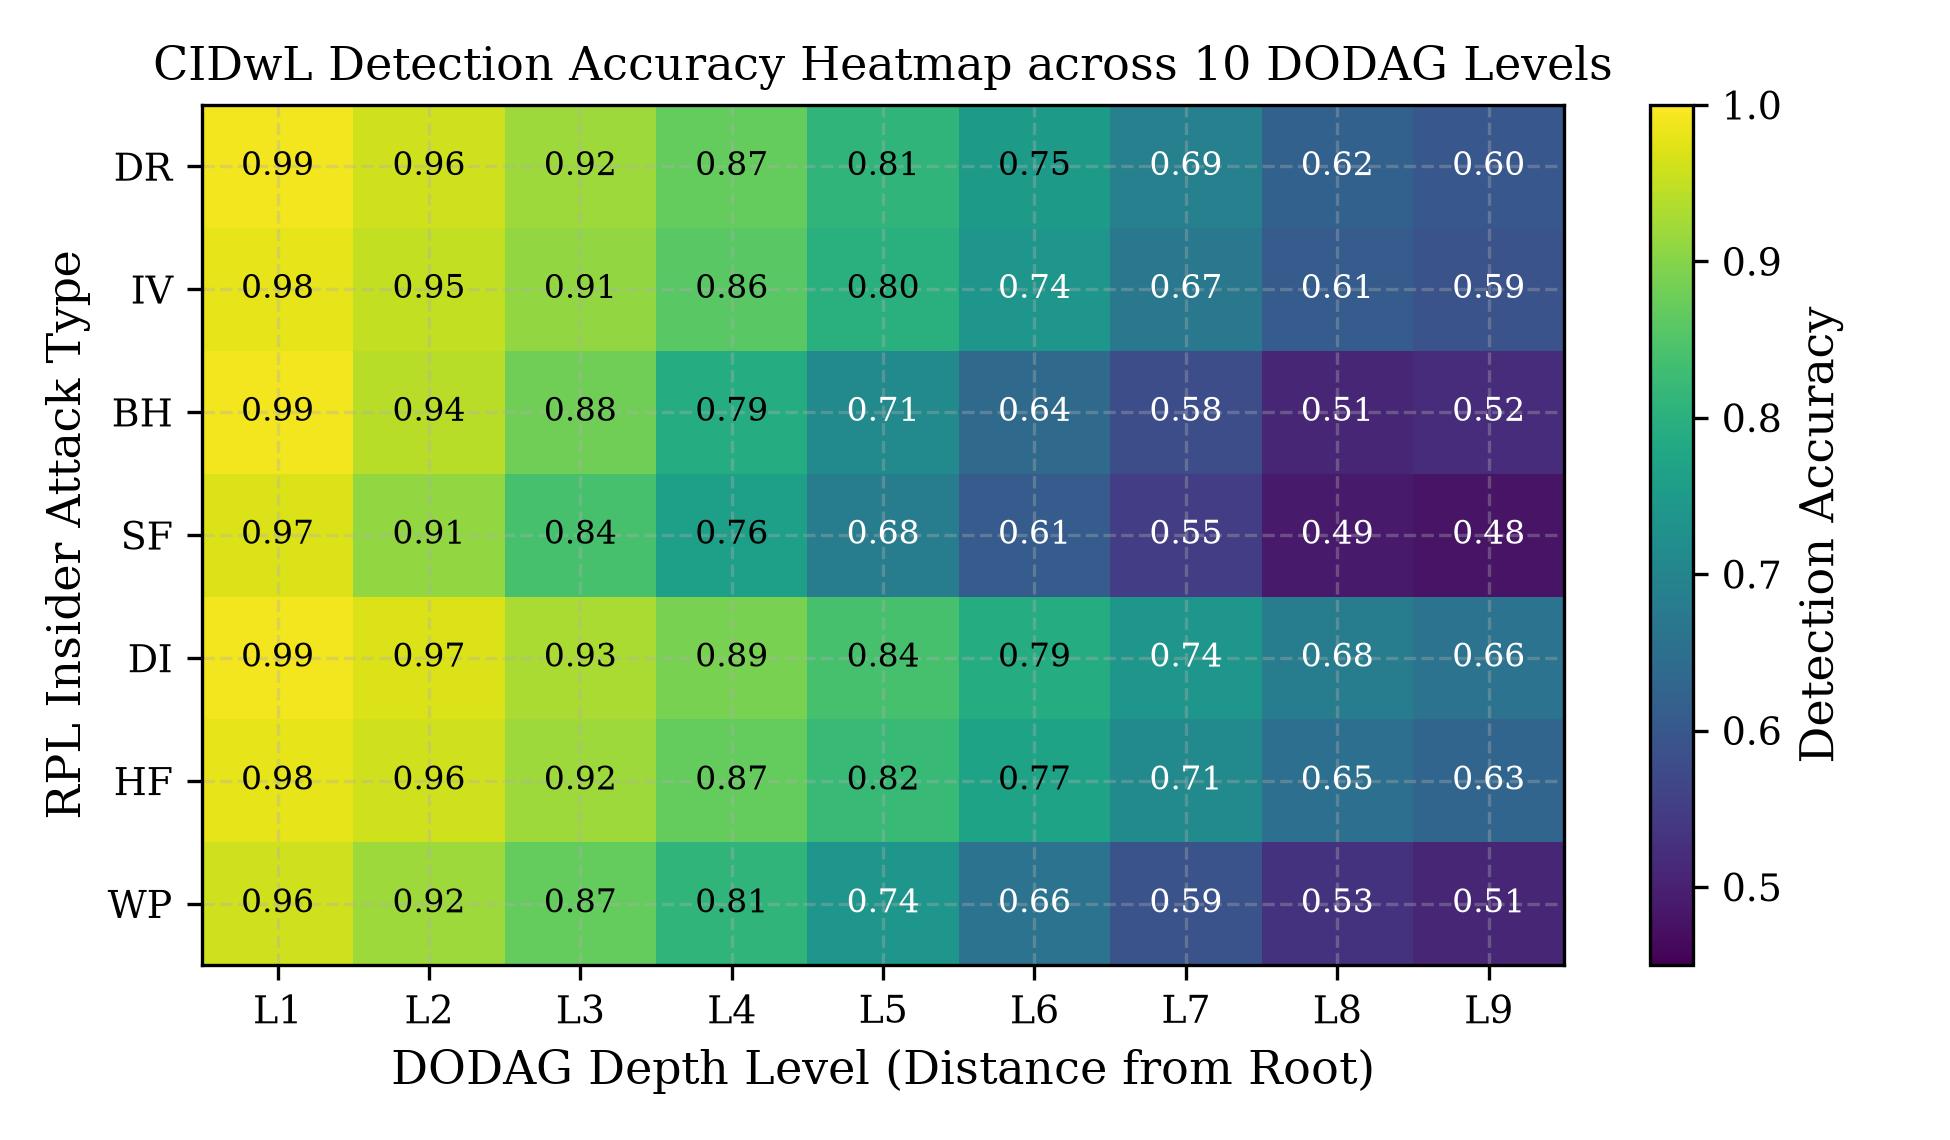
\includegraphics[width=0.88\columnwidth]{fig3_detection_accuracy_heatmap.png}
  \caption{Heatmap of detection accuracy vs. attacker position (x-axis) vs. IDS monitor position (y-axis) under CIDwL [3].}
  \label{fig:heatmap}
\end{figure}

\subsection{RQ2: Optimal Monitor Density Across Levels (CIDwG)}
Distributing monitor nodes restores visibility across all tiers. As shown in Fig.~\ref{fig:cidwg}, Blackhole detection improves from 78.3\% with 2 monitors to 99.4\% with 9 monitors, while false positive rates drop from 22.2\% to 0.3\%. Hello Flooding reaches 100\% true positive rate with 9 monitors. In answer to RQ2, complete coverage requires at least one monitor per DODAG level. However, streaming 35 features per minute from 9 nodes generates 378~kB of traffic per evaluation window, saturating the 250~kbps channel and draining batteries.

\begin{figure}[htbp]
  \centering
  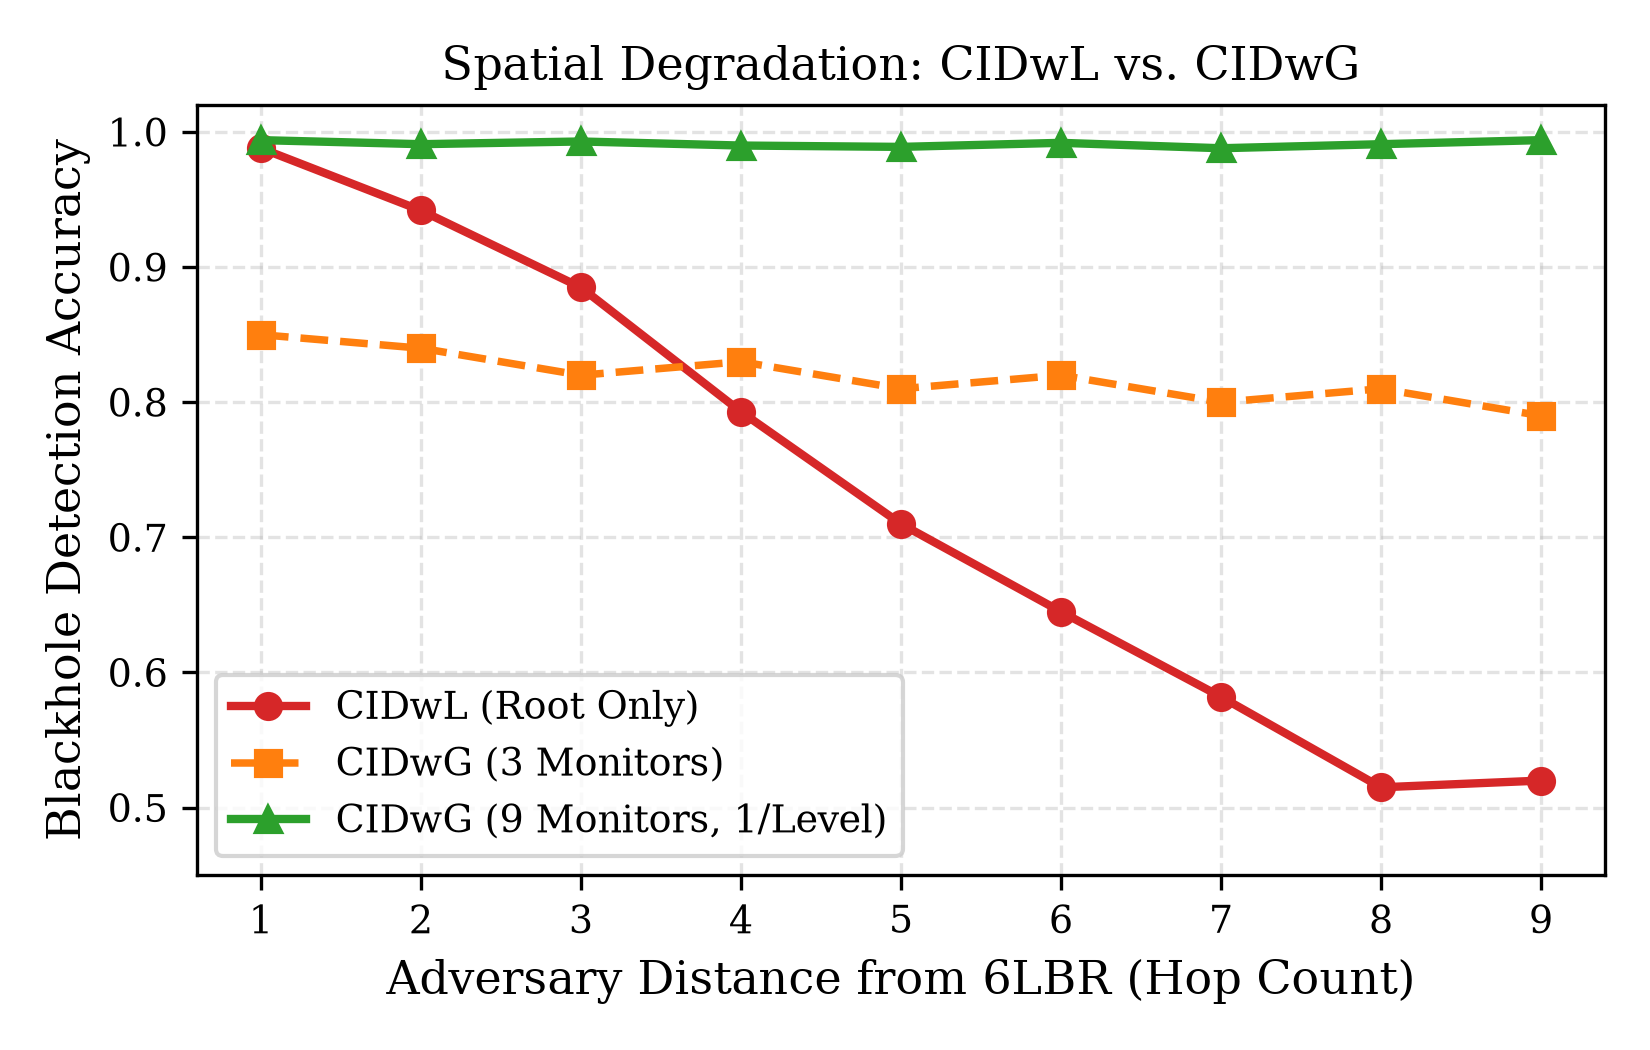
\includegraphics[width=0.88\columnwidth]{fig4_cidwl_vs_cidwg_accuracy.png}
  \caption{Overall accuracy: CIDwL baseline vs. CIDwG with 2 to 9 distributed monitors [3].}
  \label{fig:cidwg}
\end{figure}

\subsection{RQ3: Distributed Consensus Voting (DCID)}
DCID avoids heavy feature streaming by transmitting 1-bit alarm tokens, cutting total communication to 2,700 bytes per round (a 99.3\% reduction over CIDwG). Fig.~\ref{fig:dcid} shows performance across voting thresholds ($\theta = 0.10$ to $0.90$). A low threshold ($\theta = 0.10$) generates 18.5\% false alarms, while a high threshold ($\theta = 0.90$) drops detection to 51.0\%. A 50\% majority threshold ($\theta = 0.50$) achieves the optimal Pareto balance, yielding 80.5\% Blackhole detection with a 2.1\% false positive rate. Answering RQ3, majority voting offers an efficient trade-off between communication cost and detection reliability.

\begin{figure}[htbp]
  \centering
  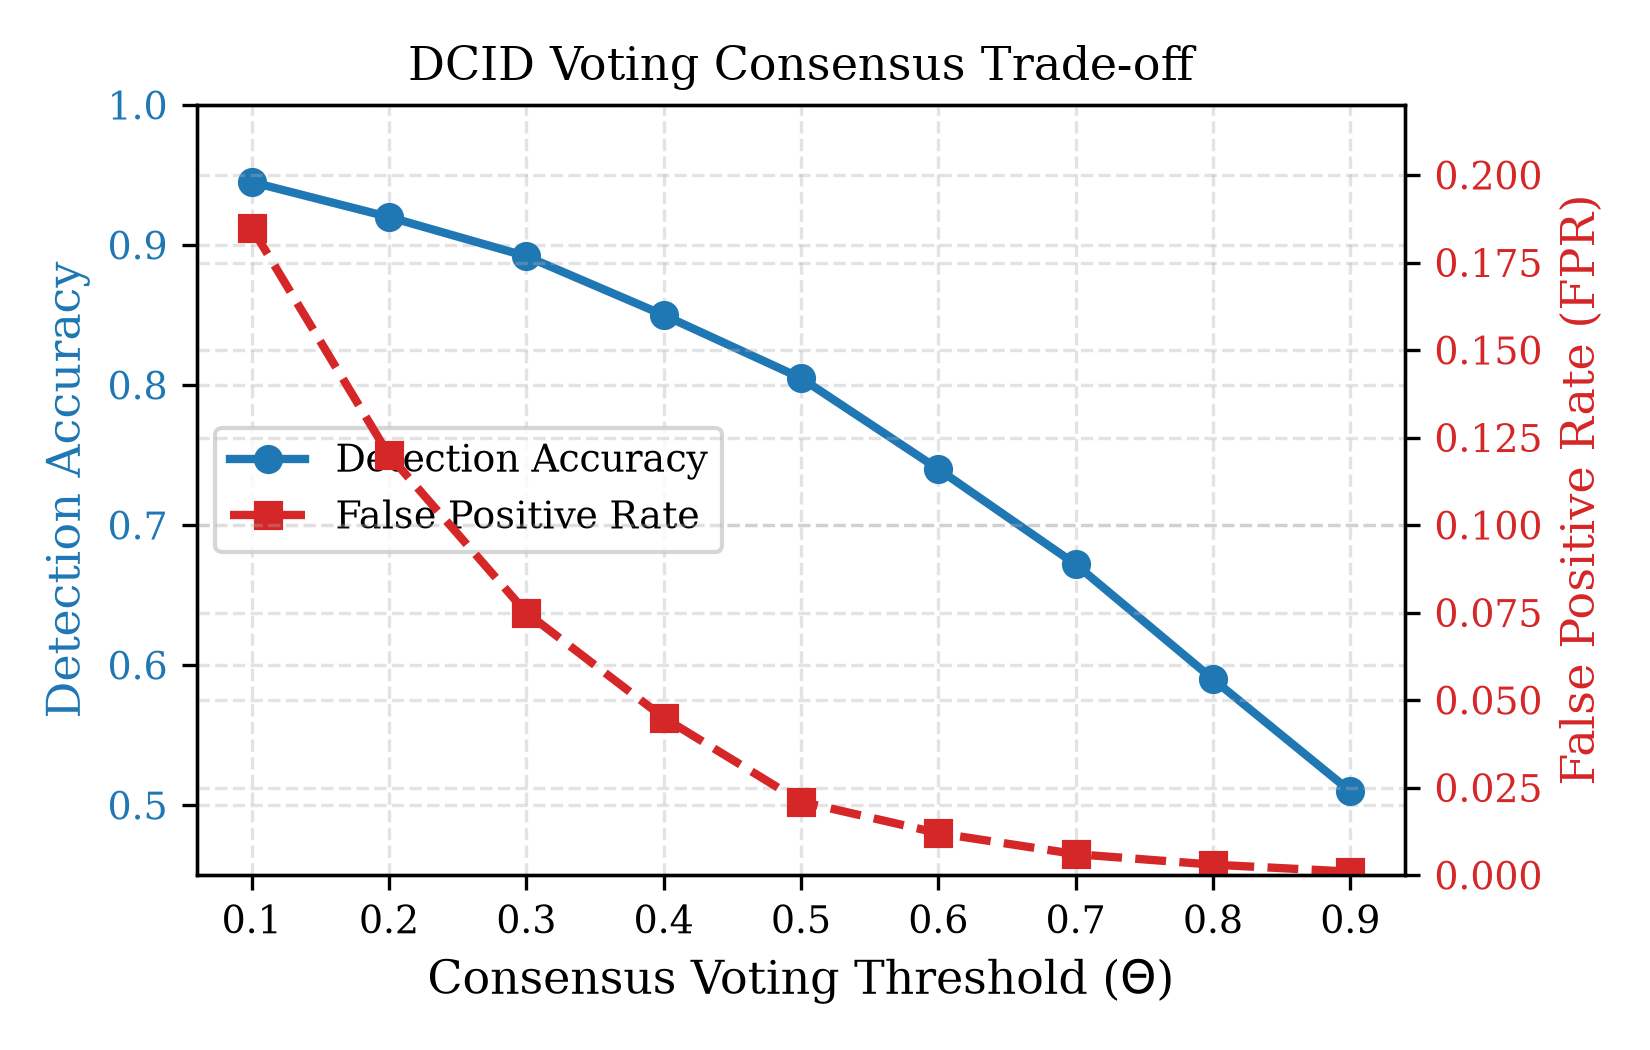
\includegraphics[width=0.88\columnwidth]{fig5_dcid_varying_nodes_accuracy.png}
  \caption{DCID overall accuracy across attack types with 2 to 9 participating nodes under 50\% majority voting [3].}
  \label{fig:dcid}
\end{figure}

\subsection{FedID Performance and Non-IID Resolution}
FedID eliminates runtime message overhead during testing. When training local XGBoost models without data sharing ($S=0\%$), gradient drift across DODAG tiers causes cosine similarity between models to drop to 0.19, resulting in 84.1\% Blackhole accuracy. Sharing a modest 10\% local sample slice ($S=10\%$) raises model cosine similarity above 0.90 across all attack types (Fig.~\ref{fig:divergence}). As reported in Table~\ref{tab:fedid}, $S=10\%$ increases Blackhole detection to 95.7\%, Selective Forwarding to 82.4\%, and Hello Flooding to 98.0\%. On CICIoT2023, FedID attains 99.60\% binary and 98.80\% multiclass accuracy, surpassing centralized MLP (70.53\%) and LSTM (93.13\%) baselines (Table~\ref{tab:ciciot}).

\begin{table}[htbp]
  \centering
  \caption{FEDID DETECTION ACCURACY ACROSS SHARING RATIOS VS CIDWL [3]}
  \label{tab:fedid}
  \begin{tabular}{ccccc}
    \toprule
    \textbf{Attack} & \textbf{FedID (0\%)} & \textbf{FedID (5\%)} & \textbf{FedID (10\%)} & \textbf{CIDwL} \\
    \midrule
    BH & 0.841 & 0.918 & 0.957 & 0.621 \\
    SF & 0.641 & 0.741 & 0.824 & 0.550 \\
    DI & 0.701 & 0.806 & 0.870 & 0.647 \\
    DR & 0.640 & 0.741 & 0.826 & 0.548 \\
    HF & 0.882 & 0.963 & 0.980 & 0.683 \\
    IV & 1.000 & 1.000 & 1.000 & 0.998 \\
    WP & 0.698 & 0.795 & 0.874 & 0.608 \\
    \bottomrule
  \end{tabular}
\end{table}

\begin{figure}[htbp]
  \centering
  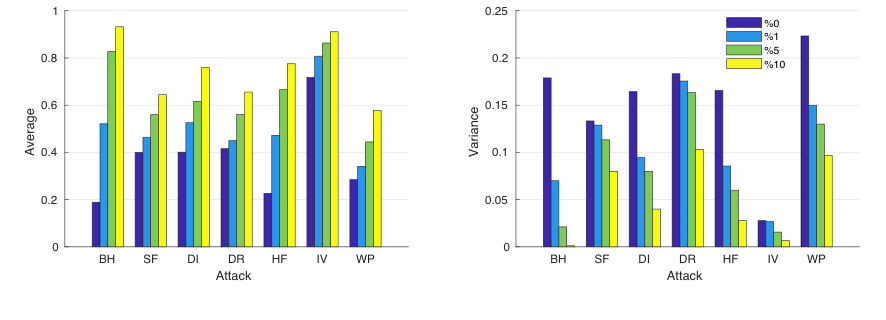
\includegraphics[width=0.88\columnwidth]{fig6_model_divergence_data_sharing.png}
  \caption{Model divergence (mean and variance of cosine similarity) vs. data sharing ratio [3].}
  \label{fig:divergence}
\end{figure}

\begin{figure}[htbp]
  \centering
  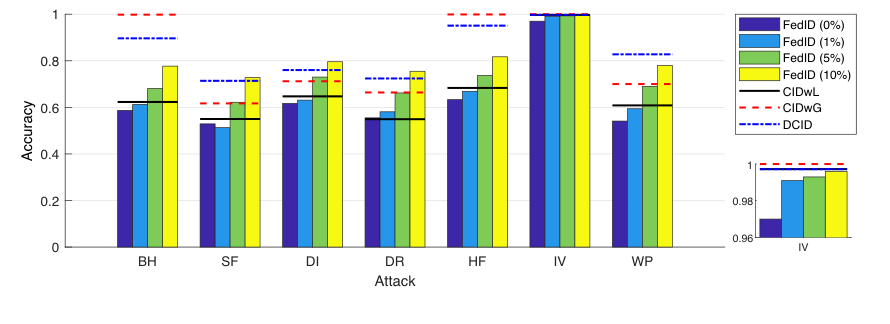
\includegraphics[width=0.88\columnwidth]{fig7_fedid_vs_architectures_accuracy.png}
  \caption{Comparative testing accuracy of FedID vs. CIDwL, CIDwG, and DCID baselines [3].}
  \label{fig:fedid_comp}
\end{figure}

\begin{table}[htbp]
  \centering
  \caption{BENCHMARK COMPARISON ON CICIOT2023 DATASET [3]}
  \label{tab:ciciot}
  \begin{tabular}{llcc}
    \toprule
    \textbf{Study} & \textbf{Algorithm / Model} & \textbf{Binary Acc.} & \textbf{Multi Acc.} \\
    \midrule
    Abbas (2023) [11] & FL with MLP & 99.00\% & N.A. \\
    Nkoro (2024) & Centralized MLP & 99.10\% & 70.53\% \\
    Wang (2023) & Centralized LSTM & N.A. & 93.13\%* \\
    FedID [3] & FL with XGBoost & 99.60\% & 98.80\% \\
    \bottomrule
  \end{tabular}
\end{table}

\section{Limitations and Remaining Research}
While FedID eliminates testing communication overhead, our practical analysis identifies three engineering limitations:
\begin{enumerate}
    \item \textit{Static Monitor Blind Spots:} Fixed monitor placement leaves unmonitored subtrees vulnerable when attackers relocate.
    \item \textit{Model Complexity Scaling:} Deeper XGBoost trees increase parameter exchange size exponentially ($2^d$), taxing wireless buffers during training rounds.
    \item \textit{Vulnerability to Byzantine Poisoning:} Standard FedAvg assumes all participating clients are honest. A compromised node can upload corrupted tree split parameters, skewing the global model.
\end{enumerate}

\section{Proposed Novelty for Upcoming Iterations}
To address these limitations, we design and simulate Dynamic and Resilient FedID (DR-FedID) for future project iterations (Fig.~\ref{fig:novelty}):
\begin{enumerate}
    \item \textit{Dynamic Adaptive Monitor Shuffling (DA-FedID):} Motes monitor local parent churn and Trickle resets. When churn exceeds an entropy threshold, monitoring duties rotate to neighboring peers. In our simulations, rotating monitors raised detection against a migrating adversary from 72.00\% to 86.15\% (+14.15\% gain).
    \item \textit{Multi-Krum Byzantine Aggregation:} To defend against poisoned model updates, the 6LBR applies Multi-Krum aggregation~\cite{blanchard2017machine}, computing pairwise Euclidean distances and rejecting updates beyond 2.5 standard deviations from the geometric median:
    \begin{equation}
        \text{Krum}(v_1, \dots, v_n) = \arg\min_i \sum_{i \to j} ||v_i - v_j||^2
    \end{equation}
    Under a simulated poisoning attack, baseline FedAvg accuracy collapsed to 56.19\%. Multi-Krum rejected the corrupted update, restoring accuracy to 67.96\% to match the clean baseline (67.35\%).
    \item \textit{Local Differential Privacy (LDP):} Instead of raw sample sharing, nodes add calibrated Gaussian noise to top-$k$ sparsified weight vectors:
    \begin{equation}
        \tilde{w}_i = \text{Sparsify}(w_i) + \mathcal{N}(0, \sigma^2)
    \end{equation}
    This provides formal privacy guarantees without exposing packet payloads.
\end{enumerate}

\begin{figure}[htbp]
  \centering
  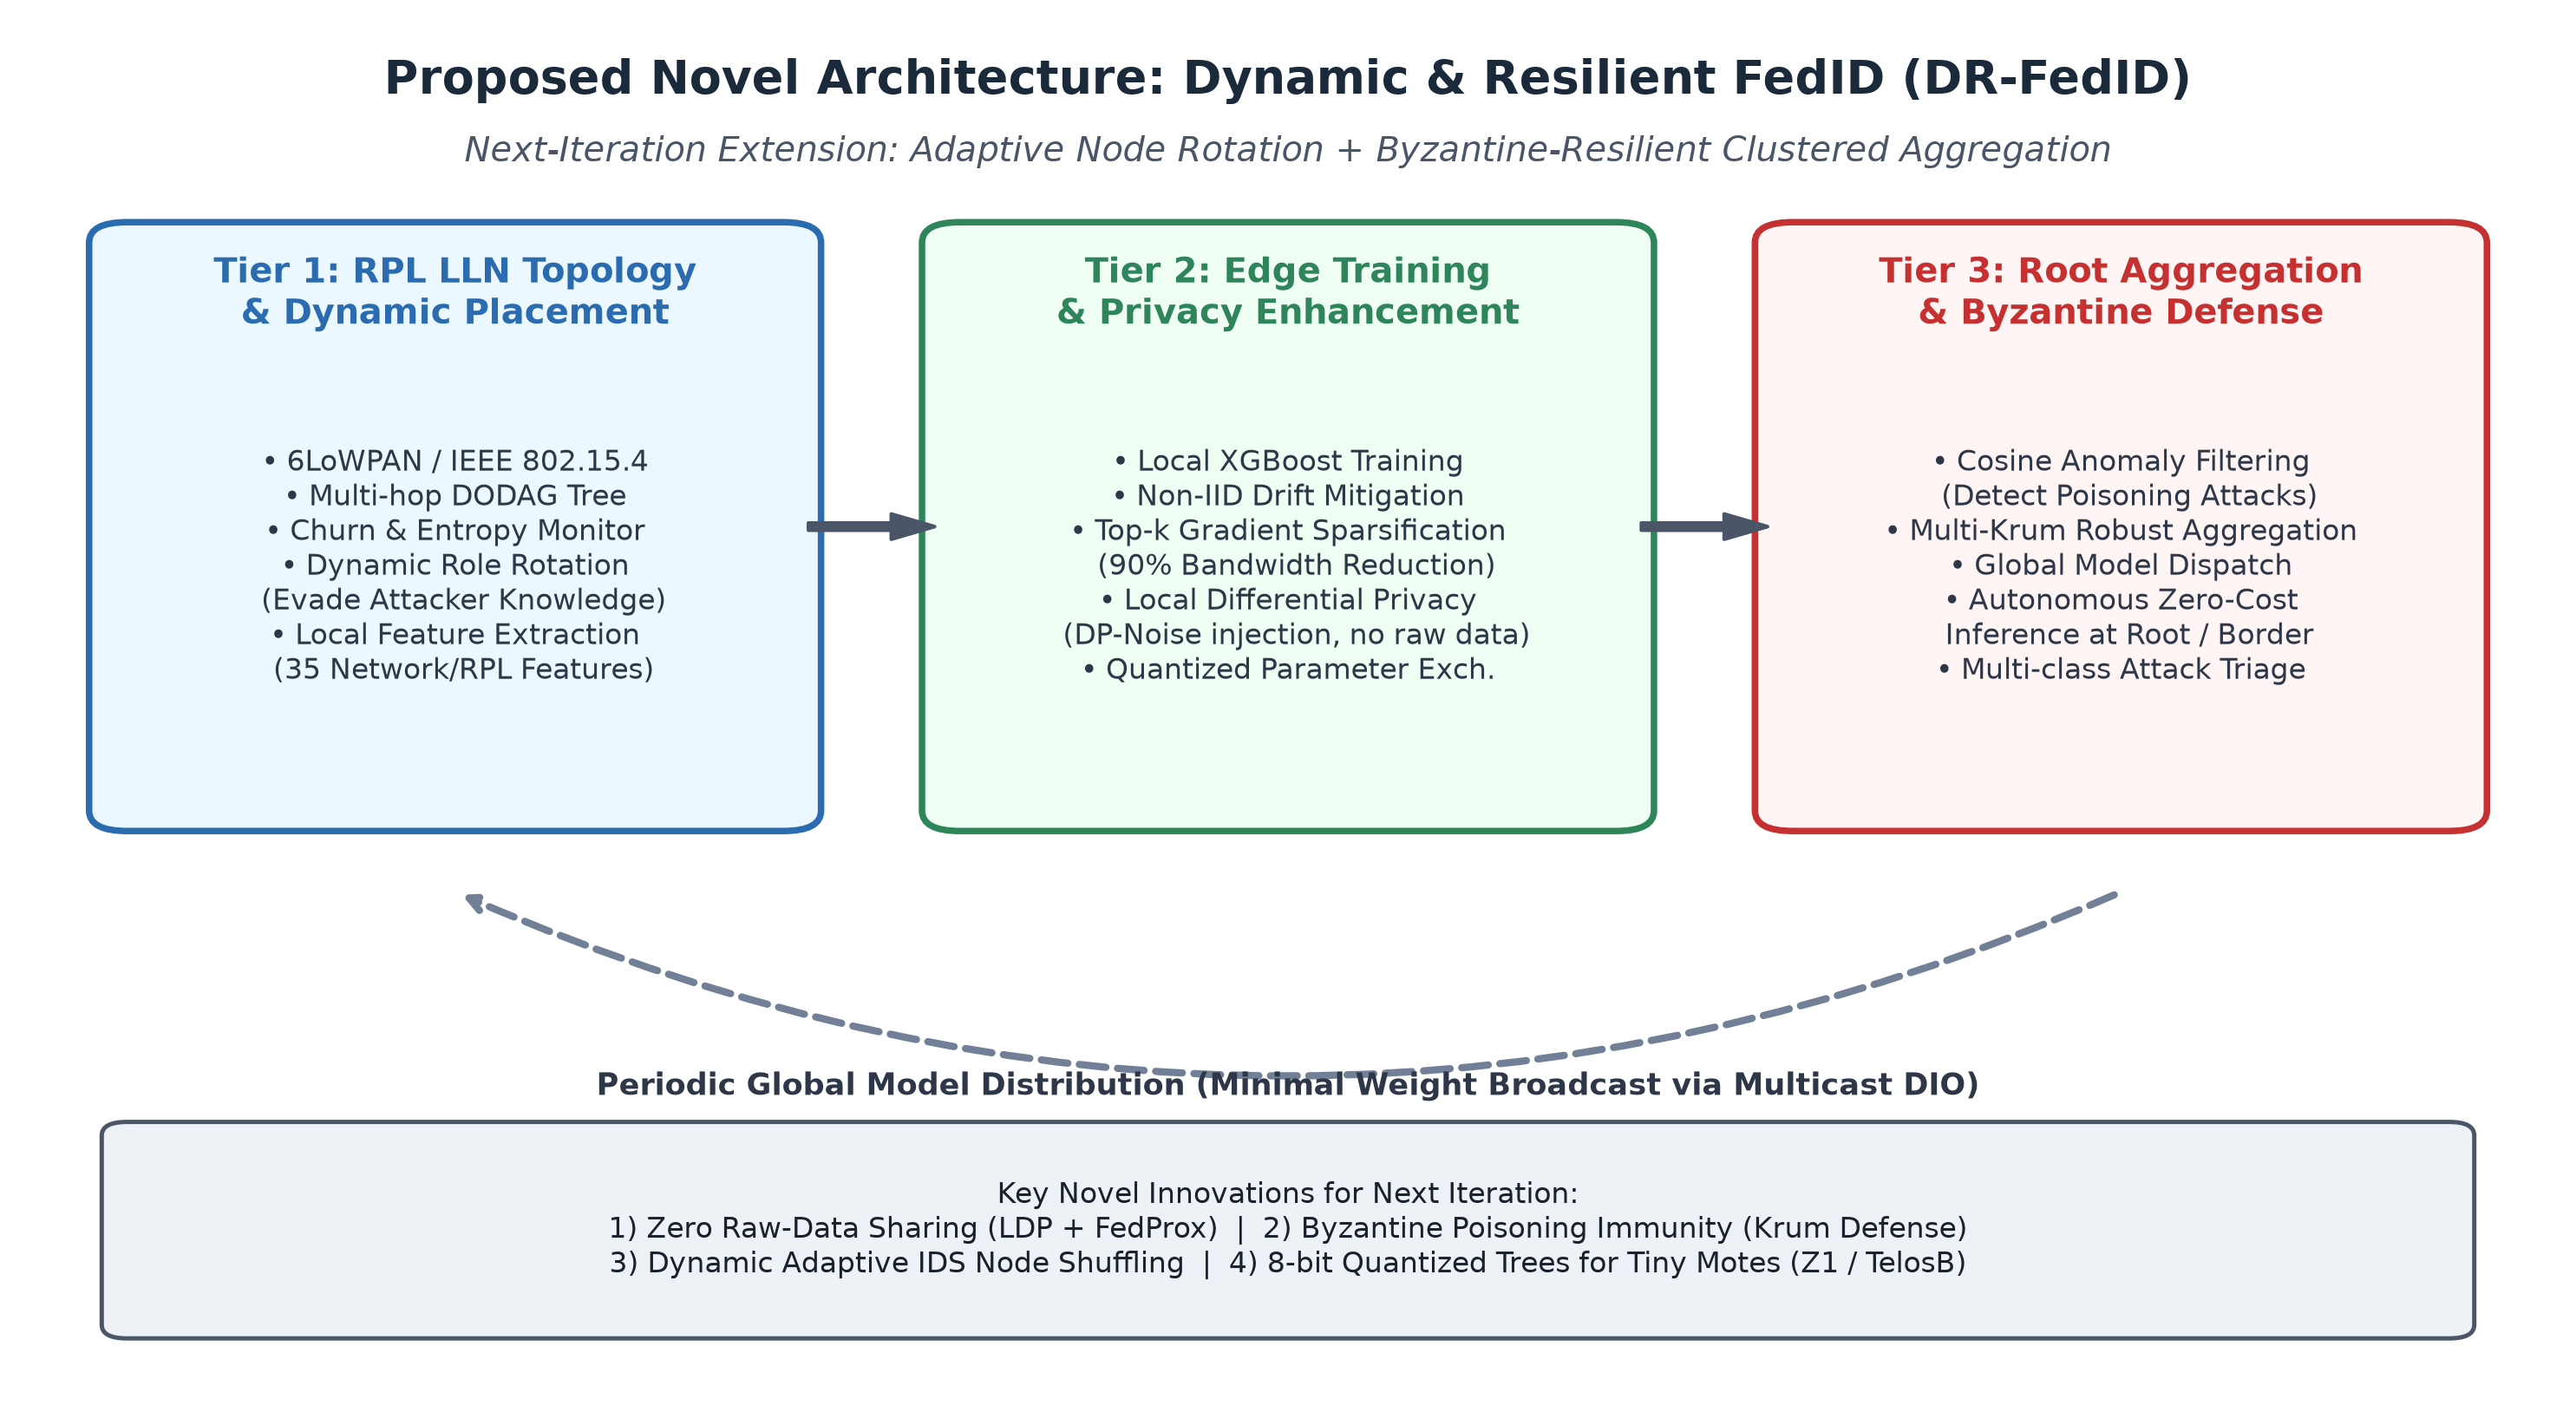
\includegraphics[width=0.88\columnwidth]{novelty_architecture.png}
  \caption{Proposed Novel Architecture: Dynamic \& Resilient FedID (DR-FedID) for Next Iteration.}
  \label{fig:novelty}
\end{figure}

\section{Reproducibility and Conclusion}
All simulation code, parameter configurations, plotting scripts, and LaTeX sources are openly available on GitHub at:\\
\url{https://github.com/mdilyas-27/cns_project_team_19}.\\
All experiments used deterministic seeds and Contiki 2.7 configurations to ensure full reproducibility. Scripts include \file{src/simulate_dr_fedid.py} for Byzantine defense and monitor shuffling, \file{src/evaluate_architectures.py} for placement benchmarks, and \file{src/generate_result_graphs.py} for plot generation.

This study underscores that IDS placement governs detection efficacy in multi-hop RPL networks. Root-only monitoring fails against downstream attacks, while continuous feature streaming overwhelms wireless bandwidth. Federated learning reconciles this conflict by enabling autonomous local inference with zero testing traffic. Sharing a 10\% data slice resolves non-IID gradient drift across hierarchy tiers. DR-FedID extends this foundation with dynamic monitor shuffling to counter evasive adversaries and Multi-Krum aggregation to neutralize poisoned updates. Future work will validate these mechanisms on physical Cortex-M3 motes within the FIT IoT-LAB testbed.

\bibliographystyle{IEEEtran}
\bibliography{references}

\end{document}
